\documentclass[conference]{IEEEtran}
\IEEEoverridecommandlockouts
% The preceding line is only needed to identify funding in the first footnote. If that is unneeded, please comment it out.
\usepackage{cite}
\usepackage{amsmath,amssymb,amsfonts}

\usepackage[linesnumbered,ruled,vlined]{algorithm2e}
\usepackage{graphicx}
\usepackage{textcomp}
\usepackage{xcolor}
\usepackage{fancyhdr} % 添加页眉页脚
\usepackage{subfigure}% in preamble

\def\BibTeX{{\rm B\kern-.05em{\sc i\kern-.025em b}\kern-.08em
    T\kern-.1667em\lower.7ex\hbox{E}\kern-.125emX}}
\begin{document}

\title{A Brief Literature Review of AI Based\\ Multimedia Technology}
\author{\IEEEauthorblockN{Zhou jy}
\IEEEauthorblockA{\textit{Department of Electrical Engineering} \\
\textit{Shanghai Jiao Tong University}\\
Shanghai, China \\
blabla@sjtu.edu.cn}

}

\maketitle
\thispagestyle{fancy} 
\lhead{} % 页眉左,需要东西的话就在{}内添加
\chead{} % 页眉中
\rhead{} % 页眉右
\lfoot{} % 页眉左
\cfoot{\thepage} % 页眉中
\rfoot{} %页眉右,\thepage 表示当前页码
\renewcommand{\headrulewidth}{0pt} %改为0pt即可去掉页眉下面的横线
\renewcommand{\footrulewidth}{0pt} %改为0pt即可去掉页脚上面的横线
\pagestyle{fancy}
\cfoot{\thepage}

\begin{abstract}
This is a literature report of the SJTU course Multimedia Communication System and Implementation EE450-1, the topic is about the AI-based multimedia technologies. I will start from the basic introduction of multimedia technology and artificial intelligence technology, in which part will briefly describe the characteristics of multimedia technology and artificial intelligence and the relationship between them; Secondly, the application of AI based multimedia technology is introduced in detail, including video streaming, congestion control, diffusion network. In each part, I will compare the similarities and differences between the traditional multimedia technology and the new AI based multimedia technology. This article is only a general exploration of the content of multimedia technologies in AI fields, and hopefully it will tighten the foundation in the field of multimedia for my further study in the future. 
\end{abstract}

\begin{IEEEkeywords}
artificial intelligence; Multimedia technology;
\end{IEEEkeywords}

\section{Brief introduction of AI based multimedia technology}\label{sec1}
\subsection{Introduction to Multimedia Technology}
Multimedia technology is a technology that uses computers to comprehensively process text, graphics, images, sound, animation, video and other information, establish logical relationships and human-computer interaction. In other words, the real multimedia technology involves the product of computer technology, while other simple things, such as movies, television, audio, etc., do not belong to the category of multimedia technology.

In the computer industry, media has two meanings: one is the carrier of information dissemination, such as language, text, image, video, audio, etc; The second is the carrier for storing information, such as ROM, RAM, tape, disk, optical disk, etc. The main carriers are CD-ROM, VCD, web pages, etc.

The media in multimedia technology mainly refers to the former definition. It refers to the use of computers to digitize text, graphics, images, animation, sound, video and other media information, and integrate them on a certain interactive interface, so that computers have the ability to interactively display different media forms. Digital media technology is mainly composed of visual presentation art and digital media application. From the perspective of media application, this technology mainly studies the methods and theories related to the processing, storage and dissemination of digital media information; From the perspective of interactive application, this technology mainly studies virtual reality technology and technology development and design; From the perspective of design, this technology mainly studies the design and production of multimedia and the integration of digital image processing and processing. Digital media technology is a new product of the combination of media and digital technology. Its application features include interest, culture and art dissemination, creativity, diversity and digitalization, among which digitalization mainly refers to the processing and access of data through simulation.

\subsection{Artificial Intelligence Technology}
Artificial intelligence technology is an advanced form of computer technology development. It fully simulates the operation process of the human brain and realizes the overall intellectualization of technology. To some extent, the application of artificial intelligence technology can also effectively reduce people's workload, and effectively reduce human errors and mistakes in work. In the process of practice, the application of artificial intelligence technology can not only carry out independent work according to procedures, but also rely on its own characteristics to carry out creative work.

Today, with the rapid and comprehensive development of digital media technology, the extensive application of artificial intelligence technology can optimize the development effect of digital media technology to a large extent. In particular, artificial intelligence can make the system have human thinking. This innovation ability is required by digital media technology. With the development of artificial intelligence technology, people begin to establish artificial intelligence learning systems, which promotes the continuous expansion of the application scope of artificial intelligence. Artificial intelligence technology can support scene interaction. For example, when this technology is applied to game design, virtual characters in the scene can gradually show a highly similar thinking mode to human work and life by simulating their behavior and continuously testing. It can be seen that the development of artificial intelligence integrates natural science, computer science and other disciplines, and fully provides interdisciplinary technical support for the development of modern computers. Therefore, it is of great significance to apply AI technology to digital media technology.

\subsection{Application of AI in Digital Media Technology}

With the rapid development of digital media technology, artificial intelligence technology has also been widely used. In digital media, artificial intelligence has a very wide range of applications. It can continuously optimize the role and efficacy of digital media, and also can improve the application advantages of digital media as a whole to meet people's needs in an all-round way. At present, the application of AI in digital media technology mainly includes the following aspects\cite{b1}.
\begin{enumerate}
\item Application of Artificial Intelligence in We-Media

\quad With the comprehensive and rapid development of information technology, a large number of We Media platforms have sprung up under the "blessing" of digital media technology, providing a platform for users to publish, share and interact information. For example, WeChat, Weibo, Today's Toutiao, Tiktok, etc., which we often use, belong to the category of We Media. In the process of continuous emergence of these We Media platforms, the scientific application of AI technology can greatly optimize the performance of the platform and better serve the majority of users.
\item Application of Artificial Intelligence in Character Design

\quad Character design is the main product of digital media technology. Before the emergence of artificial intelligence, designers may need a lot of tedious and repetitive work in the process of character design. However, relying on AI technology can effectively improve the speed and quality of character design, and can comprehensively optimize the overall effect of character design.
\item Application of Artificial Intelligence in Game Programming
    
\quad Online games are interesting projects that the majority of users are very enthusiastic about. Through artificial intelligence technology, it can provide users with rich combat roles, which in itself improves the fun of the game. At the same time, depending on AI technology, users will have different experiences each time when playing games, which can enhance their interest in war and participation.
\item Application of Artificial Intelligence in Scene Design

\quad In the process of scene design, relying on artificial intelligence technology, it can provide users with diversified choices, and can also fully feed back users' suggestions and opinions in the design process, so that users can intuitively and comprehensively observe the scene design. At the same time, the application of artificial intelligence technology has very diversified characteristics, which can serve designers and users well.
\end{enumerate}

Next, I will elaborate on the application of AI technology in video, congestion control, diffusion model and other related technologies.

\section{AI based video technology}
\subsection{Neural-Enhanced Live Streaming}

In today's Internet video, real-time video/live video occupies a large proportion. Although a lot of efforts have been made to improve the quality of user experience (QOE) in the aspects of ingest and distribution of live video, the upstream bandwidth and computing power of its streaming media have become the main factors limiting the quality of audience experience.

In the live broadcast process, it involves the process of uploading from the collection client (camera) to the server, and then sending from the server to the user. This process involves the bit rate allocation of video transmission. When the network bandwidth is small, only low-quality videos can be uploaded to the server, thus reducing the user's viewing experience (because users can only download this low-quality video).

To overcome this limitation, Kim J and his research team designed and built LiveNAS\cite{a1}, which is a new real-time video capture framework. It improves the quality of the source stream by using the computing on the capture server. The author deploys the SR model on the server side to improve the video quality. The goal of LiveNAS is to improve the video quality of the original stream on the capture server by using the super resolution based on the depth neural network, without affecting or minimizing the impact on other QoE indicators of the real-time stream, such as delay and frame loss.

\begin{figure}[!h]
\centerline{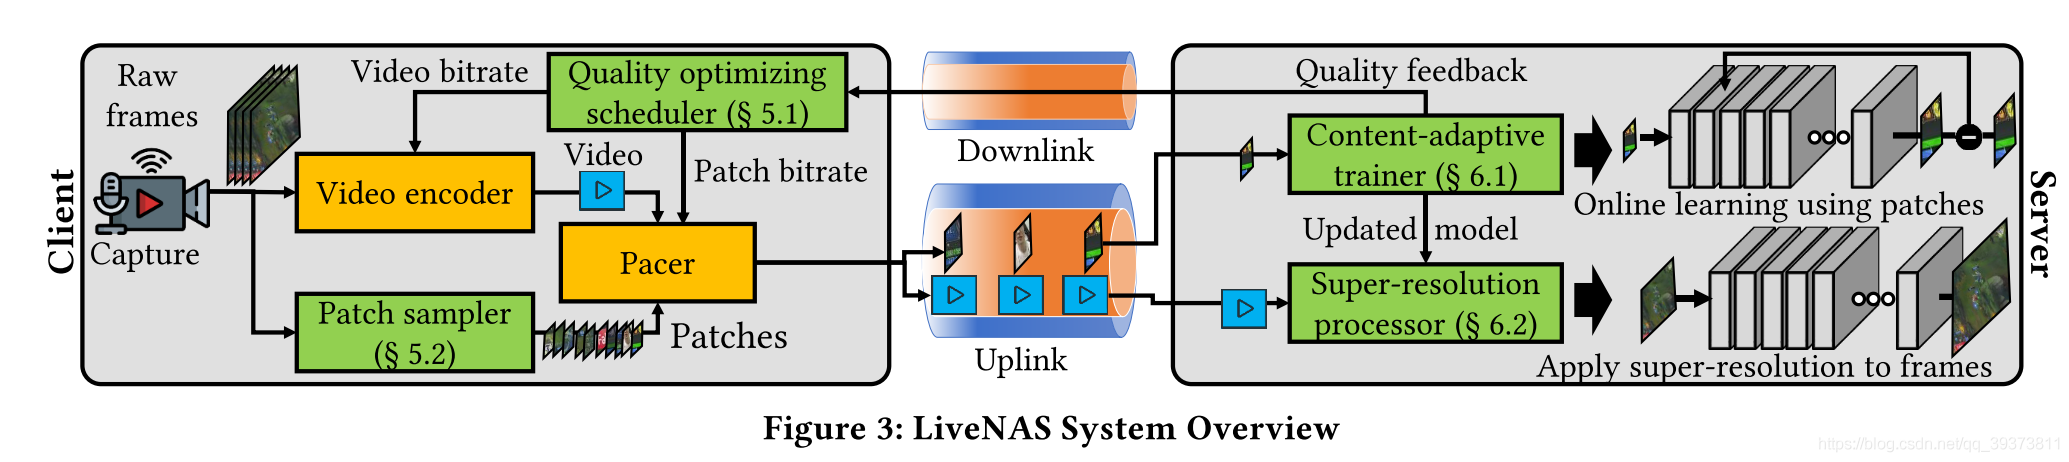
\includegraphics[scale=0.123]{picture/figure2-1.png}}
\caption{LiveNAS System Overview\cite{a1}}
\label{fig2-1}
\end{figure}

Since it is live broadcast, and the video scenes are never seen before, the CNN (SR) model needs to be retrained, that is, an online learning method is required. If the trained model is used, that is, the pre trained model, the SR effect will not be very good. Therefore, the figure \ref{fig2-1}shows the overview of LiveNAS, which is designed by the author as a collection client and a media server. A notable feature of the capture client is that it will send high-quality frame patches for online training along with the video. On the media server, online training and reasoning run in parallel. It learns the new features of online video stream, updates its mapping from low quality to high-quality version, and uses super resolution DNN to enhance the capture stream. The two design components work together on the client to maximize video quality, but there are three challenges:

\begin{enumerate}
    \item Uploading high-quality video will occupy the bandwidth of ordinary video;
    \item When training, the video SR model with little content change may converge faster; Videos with large content changes require large resources;
    \item The effect of the time difference between SR model training and inference on quality improvement should be minimized.
\end{enumerate}

In view of the above challenges, the author designed the following modules in the paper to solve the above problems:

\subsubsection{Quality-Optimizing Scheduler}\quad

The task of the Quality Optimization Scheduler is to balance the bandwidth occupied by high-quality video and real-time video, with the goal of maximizing the final video quality:

\begin{equation}
    max_{v_t,p_t}Q_{video}(v_t)+\gamma \cdot Q_{DNN}(\sum_{k=0}^t p_k),\ \ s.t.\ \forall t, \ v_t+p_t\leq C_t
\end{equation}

Where, $Q_ {video}(v_t)$indicates the quality of ordinary videos uploaded, $Q_{DNN}(\sum_ {k=0}^tp_k)$represents the quality improved by SR, $\gamma$ represents the binding factor, $v_t$ and $p_t$ is the code rate corresponding to the spectrogram video and high-quality video, and is the variable to be solved. The author uses the gradient rise method here. When the derivative is larger, it means that $p_t$ is increased as the growth of the contribution of quality. $\alpha $is the learning rate.
\begin{equation}
    p_{t+1}=\alpha\cdot\{\gamma\cdot\frac{dQ_{DNN}}{dp_t}+\frac{dQ_{video}}{dp_t} \}+p_t
\end{equation}

Seeking $dQ_{DNN}$, the author adopts the latest two $DNN$ mass change values; Seeking $dQ_{video}$, because it is nonlinear, the author observes that the same type of video is $v_t$ and $Q_{video}$ variables have similar regularization curves, so first find the regularization curve $NQ_{type}(v_t)$. Then give $v_t$, $v_{t-1}$, $Q_{video}(v_t-1) $, you can find $Q_{video}(v_t)$and its derivatives. During training, the inferred SR model parameters are synchronized every 5s and $p_t$ is updated every 1s.

\subsubsection{Patch Selection}\quad

The goal of Patch Selection is to select some high-quality video frames to upload as tags, so that the final SR can achieve the best results. The author first calculates the quality of the whole frame after encoding; Then cut a frame into $16 \times9 $block patches, and randomly select one block for each frame. Finally, select the patches whose encoded quality is lower than the overall frame quality, and then select a small number of them for transmission. Because the quality of the selected frame is low, the effect after SR processing is better.

At the same time, the transmitted patch includes its timestamp and location. The patch with a shorter time is given a higher weight during training, so that the model can better fit the latest picture.

\subsubsection{Content-Adaptive Online Learning}\quad

The purpose of this module is to suspend the training of the model and save resources when the video picture changes little, that is, when the model is fitted in advance. See the above pseudo code for details. The author has set the patience variable, when the quality between two trainings is improved $\Delta Q_{DNN}$ is less than the given threshold of $threshold_{sat}$, patient+1; When the patient reaches the given threshold of $count_{sat}$, the training will be suspended. The same goes for starting the training.
\begin{algorithm}[!h]{ %其中这里面不能有H不然会报错,不过不影响结果
	\caption{Content-Adaptive Online Training}%算法名字
	\LinesNumbered %要求显示行号
	set initial STATE as Training\;
    \Repeat{stream ends}{
	\Switch{STATE}{
       \Case{Training}{
        \For{each training epoch}{
        Compute diff of $Q_{DNN_t}$ and $Q_{DNN_{t-1}}$\;
        \If{ diff < $thresh_{sat}$}{
        $patience$ += 1\;
        \If{ $patience$ > $count_{sat}$}{
        Suspend online training\;
        STATE = Suspended\;
        $patience$ = 0\;
        }
        \Else{$patience$ = 0\;}
        }
        }
        }
        
        \Case{Suspended}{
        \For{each validation period}{
        Compute diff of $Q_{DNN_t}$ and $Q_{DNN_{t=0}}$\;
        \If{ diff < $thresh_{online}$}{
        $patience$ += 1\;
        \If{ $patience$ > $count_{online}$}{
        resume online training\;
        STATE = Training\;
        $patience$ = 0\;
        }
        \Else{$patience$ = 0\;}
        }
        }
        }
    }
    }}
\end{algorithm}

In general, in this paper, the author proposes a new real-time video capture framework, which uses the super resolution deep neural network to enhance the real-time video quality independent of the network bandwidth of the capture end; At the same time, real-time video capture is improved through online learning to solve the core challenge of using super resolution in real-time video transmission environment; LiveNAS also introduces novel design components, including quality optimization scheduler and content adaptive trainer, to fully realize the advantages of online training. LiveNAS has achieved an overall video quality improvement of 1.96 dB on average on PSNR through WebRTC in various real world network trajectories, and has brought significant (12\%$-$69\%) QoE improvement to live stream viewers.

\subsection{AI based video stream processing}
In the past video stream processing, video transmission will be compressed at the sending end, because video compression will not make much difference to the human eye. With the increasing number of cameras, the receiver may use neural networks to process video data, while the sender may use existing video compression algorithms to affect the accuracy of neural networks.

For this purpose, K Du and his research team put forward a solution in the article  upstream\cite{a2}: the sending end first sends a lower quality video to the receiving end, but at the same time, the original high-definition video receiver saves the high-definition video, processes the low quality video, and then requests the sending end to resend a specific area in the high-definition video. However, a problem encountered here is how the receiver knows which regions need high-quality video based on low-quality video. It is mentioned in the article that the neural network can also detect some large objects in low-quality video, but it does not have high accuracy for small objects. When the receiver detects small objects but is uncertain, it requests a small high-definition area from the sender. This can reduce bandwidth consumption while ensuring accuracy.

At the same time, in another paper, Li Y and his team mentioned in the paper\cite{a3} that, in order to save bandwidth, the receiver can send a function to the sender, which must be run by the sender (such as executing this function on 30 frames per second), so this function should be simple enough. At the same time, the receiver gives a threshold value. If the value calculated by the function is greater than this threshold value, the frame will be sent to the receiver. The key problem here is how the receiver determines the sending function.

If a sender can find the frame of interest according to the function, the receiver does not need to send the function. However, when the purpose of the receiver is different, or when the camera angle is different, weather conditions and environment are different, the selection of threshold and feature is different. Therefore, the receiver needs to help the sender to choose which features and thresholds to use. They proposed a reducer to determine the sending of frames through this threshold judgment, so as to reduce the bandwidth of transmitted video streams to a certain extent. The principle can be summarized as follows:

\begin{enumerate}
    \item The sender sends all frames to the receiver first.
    
    \item For each frame, the receiver passes the function and threshold value to the sender, and tells the sender the best feature and threshold value in this second. The sender only needs to filter the frame according to this rule, and the sender adds this rule to its database;
    
    \item For a new second, the sending end checks whether the characteristics are similar to the rules stored in the database. If there is a match, it extracts the frame according to the rules in the database. If not, it sends all the frames to the receiving end.
\end{enumerate}

\section{AI based congestion control technology}
\subsection{Brief Description of Congestion Control}
As a fundamental component of computer networks, Congestion Control(CC) plays a significant role in improving the network resource utilization to achieve better performance. To put it simply, if the network is likened to real road traffic, congestion control is the traffic police and traffic lights that are responsible for keeping the road from getting stuck. When some roads enter the traffic jam state, the traffic police will close the entrance of the traffic jam road and guide the traffic flow to the road without traffic jam. 

In the definition of congestion control, congestion control is mainly aimed at reliable transmission protocols such as TCP. For unreliable transmission protocols, their data integrity requirements are lower than those of reliable transmission protocols, so unreliable transmission protocols do not need congestion control. But for the information transmitted by TCP, each part of the message is connected to form a whole. Each part is indispensable. If part of the information sent is lost due to network congestion in the transmission process, the receiver will not be able to speculate about the content of the information sent from the sender.

With the emergence of a large number of new technologies and new networks, e.g., data centers (DCs), WiFi, 5G and satellite communications, the complexity and diversity of network transmission scenarios and protocols have increased dramatically. This has brought significant challenges to transmission protocol design. A rich variety of CC algorithms have been designed for specific scenarios. However, the variety of network scenarios and more importantly the intrinsic dynamics of the network, make it extremely difficult to design efficient generic CC algorithms.

Therefore, CC algorithms based on AI and ML have been proposed to provide a generic CC mechanism that could potentially underpin different network scenarios. In this part, it will give a brief description of traditional CC, AI based CC and related applications. 

\subsection{Traditional Congestion Control\cite{a4}}

Traditional CC algorithms can be divided into end-to-end CC and network assisted CC. End to end methods only require the cooperation of the sender and receiver, so they do not rely on any explicit signals from the network. Network assistant methods require the support of network devices, such as congestion information from routers. These are critical to achieving fairness and responsiveness in complex network scenarios

For end-to-end CC, one of the main challenges is to identify network congestion from implicit session signals, including packet loss and transmission delay. There are three main types of end-to-end CC methods: loss based CC, delay based CC, and hybrid CC.

Generally, based on the loss method, the transmission rate is adjusted when a given sender does not receive the corresponding ACK within a given (long) time, which usually indicates that the packet is lost. However, for some delay sensitive applications, lower transmission time cannot be guaranteed. In addition, packet loss may not be caused by network congestion (for example, random packet loss), which may mislead any CC decision.

Therefore, a delay based method is proposed, which depends on the detected transmission delay caused by the network. Compared with loss based methods, delay based methods are more suitable for high-speed and flexible networks, such as wireless networks, because they are not affected by random packet loss. However, calculating accurate transmission delay is still a major challenge. For example, a small change in the packet processing time in the host stack may lead to a deviation in the measured transmission delay, resulting in an erroneous decision related to the transmission rate. 

And the hybrid method is formed by making full use of the advantages of the above two methods. However, the hybrid method cannot accurately identify the network state based on the implicit signals related to packet loss and transmission delay.

In order to solve these problems, network assisted CC method was proposed. The network equipment provides explicit signals related to network status for host to make transmission rate decisions.

The above is a brief introduction to the traditional CC algorithm. With the emergence of a large number of new technologies and networks such as data center, WiFi, 5G, satellite communication, etc., the complexity and diversity of network transmission scenarios have increased dramatically. This brings great challenges to CC. The traditional CC method may be good in a certain scenario, but it cannot guarantee the performance in different network scenarios. In addition, changing traffic patterns in a network scenario may also affect the performance of the solution. Therefore, an intelligent CC method is needed.
\subsection{Learning-based Congestion Control}

In order to solve the above problems, a learning based CC algorithm is proposed. Different from the traditional CC algorithm, the learning based scheme is based on real-time network state to make control decisions, rather than using predetermined rules. This makes them have better adaptability to dynamic and complex network scenarios.

According to different mechanisms, learning based CC algorithms can be divided into two categories: performance oriented CC algorithms and data-driven CC algorithms. The performance oriented CC algorithm uses the objective optimization method to train the model and get the output. Such algorithms generally require manual determination of the parameters in the utility function. The learning process should converge to the optimal value of the utility function.

Next, we will mainly introduce some typical performance oriented CC algorithms.
\subsubsection{Remy Algorithm}\quad

Remy\cite{a5} is an early version of the performance oriented CC algorithm. Its utility function consists of throughput and latency. In order to maximize the expected value of the utility function, Remy looks up the mapping according to the pre calculated lookup table. Accordingly, the corresponding transmission rate is estimated. Remy is mainly composed of the following modules: 

\begin{enumerate}
    \item A priori hypothesis model

    \quad If we assume that the state in the network conforms to the Markov process, that is, the future state in the network is only related to the current state. For example, we can take three states in the network as the input of the Markov chain: bottleneck link speed (C), propagation delay (D), and link reuse (N). We can infer the state evolution of the network in the future.
    \item Flow model

    \quad In terms of traffic model, the author simply takes the switch model of bell link switch as an example. In other words, the sending and non sending data in the network follow a random process. The "open" action is subject to exponential distribution, and the "close" action is subject to empirical distribution
    \begin{figure}[!h]
    \centerline{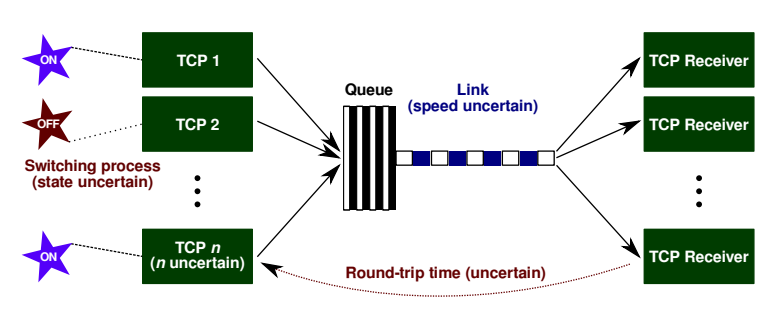
\includegraphics[scale=0.25]{picture/figure3-1.png}}
    \caption{Dumbbell network with uncertainty.\cite{a5}}
    \label{fig3-1}
    \end{figure}
    \item objective function

    \quad The objective function is written as follows:
    \begin{equation}
        Alpha-fairness metric\ U_\alpha(x)=\frac{x^{1-\alpha}}{1-\alpha}
    \end{equation}
    \quad $\alpha$ in the objective function formula represents a balance coefficient, and $x$ represents the throughput of the machine. Each terminal uses the network status information to calculate the current objective function value, that is, $U(x)$. Generally speaking, the larger $U(x)$, the better. $\alpha$ Take different values to indicate that different weights of $x$ are taken into account in the objective function value.

    \quad For example, when $\alpha=1$, only $x$ throughput is considered and no other parameters are considered. In this way, the value of the objective function is only related to $x$. In this way, the purpose of each terminal is to maximize its score as much as possible, and the means is to improve its throughput. However, for a best effort network like TCP, the network system may collapse if each terminal blindly increases its throughput. In order to balance individual and overall, fairness and efficiency, the author proposes an improved objective function:
    \begin{equation}
        U_\alpha(x)-\delta U_\beta(x)=\frac{x^{1-\alpha}}{1-\alpha}-\delta\frac{\gamma^{1-\beta}}{1-\beta}
    \end{equation}
    
    \quad In this function, we no longer only consider throughput, but also consider link delay. However, the objective function principle remains unchanged, and the function value should be improved as much as possible. So the purpose of Remy is to find out what algorithm can realize your values. $\beta$ is like $\alpha$, $\delta$ represents the importance of throughput and delay.

    \quad The following figure shows the overall model of Remy algorithm:
    \begin{figure}[!h]
    \centerline{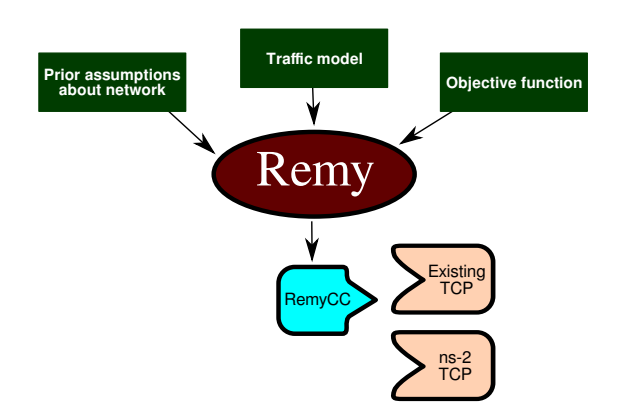
\includegraphics[scale=0.25]{picture/figure3-2.png}}
    \caption{Remy's schemes for congestion control.\cite{a5}}
    \label{fig3-2}
    \end{figure}   
\end{enumerate}

\subsubsection{PCC Vivace Algorithm}\quad

PCC uses the black box method. The core idea is to perceive the performance of the network after a certain transmission rate is given, so as to adjust the transmission rate. Traditional PCC Allegro observes the performance indicators generated by sending at a specific rate through the sender, converts the indicators into corresponding effective values, and then adjusts the sending rate to a more efficient direction according to experience. The design of Pcc IVace combines the basic framework of PCC Allegro and the principle of online learning in machine learning to solve the network congestion control problem by adjusting the direction, step size and threshold of the sending rate. PCC and PCC Vivace are both designed based on practical functions covering basic performance indicators such as round trip time (RTT), and have also shown excellent performance. Here is a brief introduction:

PCC Allegro\cite{a6} divides time into continuous monitor intervals (MIs), and the degree of MI is usually 1 to 2 RTTs. PCC selects a transmission rate $r$ in an MI, and sends at this rate in this MI. After about one RTT, the sender will see the SACK. PCC converts these ACK information into performance evaluation indicators such as throughput, packet loss rate, and delay. These indicators calculate a utility value through a utility function, expressed in $u$.

At a rate $r$, PCC will try $(1+\epsilon)*r$ and $(1-\epsilon)r$ The rate of $r$. PCC will move towards higher utility value. To reduce some test noise, PCC does not use the method of testing in two MI, but tests two different rates in a random sequence in four MI. If both sides get higher utility values, PCC chooses one of the random values as the next transmission efficiency. In a network with $n$ senders, the maximum bandwidth of the network is $C$, and the utility function of each sender $i$ is:
\begin{equation}
    u_i(x_i)=T_i* Sigmoid_\alpha(L_i-0.05)-x_i * L_i
\end{equation}

Where, $x_i$ is the transmission rate of the transmitter $i$, $L_i$ is the observed packet loss rate, $T_i=x_i* (1-L_i)$.

The control algorithm steps of PCC can be divided into the following starting states and decision-making states:
\begin{enumerate}
    \item Starting State

    \quad The startup transmission rate is set to $2*\frac{MSS}{RTT}$, and then the transmission rate is doubled in each subsequent MI. The PCC termination start phase is not determined by packet loss, but when the calculated utility value decreases;
    \item Decision Making State

    \quad PCC selects 4 MI and divides them into 2 groups (randomly). One group is sent at the rate of $r(1+\epsilon)$, the other is at $r(1-\epsilon)$. After sending, the calculated utility values are recorded as $Ui+$, $Ui-$. If $Ui+>Ui-$, the new rate is set to $r(1+\epsilon)$. On the contrary, set $r(1-\epsilon)$. However, if the utility decreases, PCC will keep its rate at the current rate as $\epsilon=\epsilon+\epsilon_{min}$, but the maximum difference is more than $\epsilon_{max}$. Here it uses $\epsilon_{min}= 0.01$, $\epsilon_{max}=0.05$.
\end{enumerate}

PPC Vivace algorithm\cite{a7} optimizes and improves PCC Allegro algorithm. The core of its improvement includes: using a new learning framework to ensure that multiple Vivace flows can converge to a fair and efficient state; A gradient based online optimization algorithm is used to adjust the transmission rate, which will calculate the step size.

PCC Vivace's utility function framework can be evaluated as: 
\begin{equation}
    u(x_i,\frac{d(RTT_i)}{dT},L_i)=x_i^t-bx_i\frac{d(RTT_i)}{dT}-cx_i\* L_i
\end{equation}

Where $0<t<1$, $b>=0$, $c>0$, ($b$, $c$, $t$ are constants) The first term of the objective function is the power of the transmission rate, the second term is the proportional term of the RTT gradient, and the third term is the proportional term of the packet loss rate. Compared with Allegro, we can see that Vivace considers the time delay (the second term) in the objective function. In general, utility value is rewarded when throughput increases, and punished when RTT and packet loss rate increase.

\subsubsection{Other algorithms}\quad

As is mentioned before, learning-based CC algorithms can be divided into two groups: performance-oriented CC algorithms and data-driven CC algorithms. The Remy algorithm and PCC algorithm mentioned earlier belong to performance-oriented CC algorithms. 

Other performance-oriented algorithms like GCC and Copa. GCC Algorithm adopts Kalman filtering, which is a method of using the linear system state equation to optimally estimate the system state through the observation data. Based on Kalman filter, GCC estimates end-to-end one-way delay change and dynamically controls transmission rate. Copa optimizes the objective function and adjusts the transmission rate according to the current throughput and packet delay. Compared with the performance oriented CC algorithm mentioned earlier, the data-driven CC algorithm is more dependent on data sets and has convergence problems. However, because the data-driven CC algorithm updates the parameters according to the current data rather than relying on the given constant parameters, it has stronger adaptability and can meet different network scenarios through learning. 

In addition, mainstream research focuses more on data-driven CC algorithm. For data-driven CC algorithm, machine learning technology is used for model training, including supervised learning technology, unsupervised learning technology and RL technology. Supervised learning and unsupervised learning technologies are widely used to improve network CC. However, these schemes are only partially successful because they are offline training and cannot classify the actual wireless and congestion losses. 

As a result, learning based CC is still in its infancy. Most learning based CC algorithms control the sending rate by adjusting the congestion window (CWND), rather than directly adjusting the sending rate. Therefore, burst is still a problem in high-speed networks. Designing a universal learning based CC scheme that can work in real network scenarios is still the main goal of academia and industry.

\section{Diffusion Models\cite{a8}}
Diffusion models are new SOTA in depth generation models. The diffusion model surpasses the original SOTA: GAN in the image generation task, and has excellent performance in many application fields, such as computer vision, NLP, waveform signal processing, multimodal modeling, molecular graph modeling, time series modeling, adversarial purification, etc. In addition, diffusion models are closely related to other research fields, such as robust learning, representation learning, and reinforcement learning.
\subsection{Traditional diffusion model}
A core problem of generative modeling is the tradeoff between flexibility and computability of the model. The basic idea of diffusion model is to systematically disturb the distribution of data by forward diffusion process, and then recover the distribution of data by learning the reverse diffusion process, thus creating a highly flexible and easy to calculate generation model.

\subsubsection{Denoising Diffusion Probabilistic Models (DDPM) }\quad

A DDPM consists of two parameterized Markov chains, and uses variational inference to generate samples consistent with the original data distribution after a finite time. The function of the forward chain is to disturb the data. It gradually adds Gaussian noise to the data according to the pre designed noise progress until the distribution of the data tends to a prior distribution, that is, the standard Gaussian distribution. The reverse chain starts from the given prior and uses the parameterized Gaussian transform kernel to learn to gradually restore the original data distribution.

\subsubsection{Score-Based Generative Models (SGM) }\quad

The above DDPM can be considered as a discrete form of SGM. SGM constructs a stochastic differential equation (SDE) to smooth the data distribution and transform the original data distribution into a known prior distribution:

\begin{equation}
    dxf(x,t)dt+g(t)dw
\end{equation}

And a corresponding reverse SDE to transform the prior distribution back to the original data distribution:
\begin{equation}
    dx=f(x,t)-g(t)^2\nabla_x logq_t(x)dt+g(t)dw
\end{equation}

Therefore, to reverse the diffusion process and generate data, the only information need is the fractional function at each time point. Using the score matching technique, it can learn the score function through a certain loss function. 

However, the original diffusion model also has shortcomings. Its sampling speed is slow, and it usually requires thousands of evaluation steps to extract a sample; Its maximum likelihood estimation cannot be compared with the model based on likelihood; It has poor ability to generalize to various data types. Nowadays, many researches have made many efforts to solve the above limitations from the perspective of practical application, or analyzed the model capability from the perspective of theory. The improvement research on diffusion models is divided into three corresponding categories: sampling speed enhancement, maximum likelihood enhancement and data generalization enhancement. The improved diffusion models will be described later.

\subsection{Sampling acceleration method}

In application, in order to optimize the quality of new samples, diffusion models often require thousands of steps of calculation to obtain a new sample. This limits the practical application value of the diffusion model, because in practical application, we often need to generate a large number of new samples to provide materials for the next step of processing. Researchers have done a lot of research on improving the sampling speed of the diffusion model. It can be classified into three methods: Discretionation Optimization, Non Markovian Process, and Partial Sampling.

\subsubsection{Discretization Optimization}\quad

This method optimizes the method for solving the diffusion SDE. In reality, only discrete solutions can be used to approximate the real solution to solve complex SDE, so this kind of method tries to optimize the discretization method of SDE, and reduce the number of walks while ensuring the sample quality. SGM proposes a general method to solve the inverse process, that is, the same discrete method is adopted for the forward and backward processes. If the discrete mode of forward SDE is given:

\begin{equation}
    x_{i+1}=x_i+f_i(x_i)+g_iz_i,\ i=0,1,\cdots,N-1
\end{equation}

Then we can discretize the reverse SDE in the same way:

\begin{equation}
    x_i=x_{i+1}-f_{i+1}(x_{i+1})+g_{i+1}g_{i+1}^ts_\theta * (x_{i+1},i+1)+g_{i+1}z
\end{equation}

This method is slightly better than simple DDPM. Further, SGM added a corrector to the SDE solver, so that the samples generated in each step have the correct distribution. At each step of the solution, after the solver gives a sample, the corrector uses the Markov chain Monte Carlo method to correct the distribution of the sample just generated. The experiment shows that adding correctors to the solver is more efficient than directly increasing the steps of the solver.

\subsubsection{Non-Markovian Process}\quad

This method breaks through the limitation of the original Markovian Process. Each step of its inverse process can rely on more previous samples to predict new samples, so it can also make better predictions when the step size is large, thus speeding up the sampling process. DDIM, the main work, no longer assumes that the forward process is a Markov process. The sampling process of DDIM can be regarded as a discretized divine ordinary differential equation, which is more efficient and supports sample interpolation. Further research shows that DDIM can be regarded as a special case of the diffusion model PNDM on manifolds.

\subsubsection{Partial Sampling}\quad

This method directly reduces the sampling time by ignoring some time nodes in the generation process and only using the remaining time nodes to generate samples. For example, Progressive Distillation distills a more efficient diffusion model from the trained diffusion model. For a trained diffusion model, Progressive Diffusion will train a new diffusion model, so that one step of the new diffusion model corresponds to two steps of the trained diffusion model, so that the new model can save half of the sampling process of the old model. Continuously circulating the distillation process can make the sampling step exponentially lower.The specific algorithm is as follows:
\begin{algorithm}[!h]{ %其中这里面不能有H不然会报错,不过不影响结果
	\caption{Progressive distillation}%算法名字
 \textbf{Require:} Trained tescher model $\hat{x}_\eta(z_t)$\;
 \textbf{Require:} Data set $D$\;
 \textbf{Require:} Loss weight function w()\;
 \textbf{Require:} Student sampling steps $N$\;
\LinesNumbered %要求显示行号
\For{K iterations}{
$\theta\longleftarrow \eta$ \quad $\lhd$ Init student from teacher\;
\While{not converged}{
x$\sim D$\;
t = i / N,\ \ i $\sim Cat[1,2,\dots,N]$\;
$\epsilon\sim N(0,I)$\;
$z_t=\alpha_t x+\sigma_t\epsilon$\;
$\#$ 2 steps of DDIM with teacher\;
$t'=t-0.5/N, t''=t-1/N$\;
$z_{t'}=\alpha_{t'}\hat{x}\eta(z_t)+\frac{\sigma_{t'}}{\sigma_t}(z_t-\alpha_{t}\hat{x}_\eta(z_t))$\;
$z_{t''}=\alpha_{t''}\hat{x}\eta(z_{t'})+\frac{\sigma_{t''}}{\sigma_{t'}}(z_{t'}-\alpha_{t'}\hat{x}_\eta(z_{t'}))$\;
$\hat{x}=\frac{z_{t''}-(\sigma_{t''}/\sigma_t)z_t}{\alpha_{t''}-(\sigma_{t''}/\sigma_t)\alpha_t}$\quad $\rhd$ Teacher $\hat{x}$ target\;
$\lambda_t=log[\alpha_t^2/\sigma_t^2]$\;
$L_\theta=\omega(\lambda_t)||\hat{x}-\hat{x}\theta(z_t)||_2^2$\;
$\theta\longleftarrow\theta-\gamma\nabla_\theta L_\theta$\;
}
$\eta\longleftarrow\theta$\quad$\rhd$ Student becomes next teacher\;
$N\longleftarrow N/2$\quad$\rhd$ Halve number of sampling steps\;
}
}
\end{algorithm}

\subsection{Maximum likelihood estimation esnhancement}

Diffusion model performs worse in maximum likelihood estimation than generation model based on likelihood function, but maximum likelihood estimation is significant in many application scenarios, such as image compression, semi supervised learning, and adversarial purification. Since it is difficult to calculate the log likelihood directly, the research mainly focuses on the optimization and analysis of the lower bound of variation (VLB). We elaborate on the model to improve the maximum likelihood estimation of the diffusion model. We classify them into three categories: Objectives Designing, Noise Schedule Optimization, and Learning Reverse Variance.

\subsubsection{Objectives Designing}\quad

This method uses diffusion SDE to deduce the relationship between the logarithmic likelihood of birth data and the loss function of fractional function matching. By properly designing the loss function, VLB and log likelihood can be maximized. The loss function fitted by the fractional function is as follows:

\begin{equation}
\begin{aligned}
    J_{DSM}(\theta;\lambda(\cdot)):=\frac{1}{2}\int_0^TE_{p(x)p_{0t}(x'|x)}[\lambda(t)||\nabla_{x'}logp_{0t}(x'|x)\\
    -s_\theta(x',t)||_2^2]dt
\end{aligned}
\end{equation}

\subsubsection{Noise Schedule Optimization}\quad

This method increases VLB by designing or learning the noise progress of the forward process. When the number of walks is close to infinity, the loss function is completely determined by the endpoint of the signal to noise ratio function SNR (t):

\begin{equation}
    L_\infty(x)=\frac{1}{2}E_{\epsilon\sim N(0,I)}\int_{SNR_{min}}^{SNR_{max}}||x-\hat{x}\theta(z_v,v)||_2^2dv
\end{equation}

\subsubsection{Learnable Reverse Variance}\quad

This method learns the variance of the reverse process, and can reduce the fitting error and effectively maximize VLB under the condition of a given forward process.

\subsection{Data generalization enhancement}

The diffusion model assumes that the data exists in Euclidean space, that is, a manifold with plane geometry, and adding Gaussian noise will inevitably convert the data into continuous state space. Therefore, the diffusion model can only process continuous data such as images at first, and the effect of directly applying discrete data or other data types is poor. This limits the application scenarios of the diffusion model. Several studies have extended the diffusion model to other data types, and we have explained these methods in detail. We subdivide it into two types of methods: Feature Space Unification and Data Dependent Transition Kernels.

\subsubsection{Feature Space Unification}

This method converts the data into a unified latent space, and then spreads it on the latent space. LSGM proposes to convert the data to the continuous late space through the VAE framework, and then spread it on it. The difficulty of this method is how to train VAE and diffusion model at the same time. LSGM indicates that because the potential prior is intractable, the score matching loss is no longer applicable. LSGM directly uses the traditional loss function ELBO in VAE as the loss function, and derives the relationship between ELBO and score matching:
\begin{equation}
\begin{aligned}
    CE(q((z_0|x)||p(z_0))=E_{t\sim U[0,1]}[\frac{g(t)^2}{2}E_{q(z_t,z_0|x)}\\
    [||\nabla_{z_t}logq(z_t|z_0)-\nabla_{z_t}logp(z_t)||_2^2]]
\end{aligned}
\end{equation}

This equation holds in the sense of ignoring constants. LSGM can efficiently learn and optimize ELBO by parameterizing the fractional function of samples in the diffusion process.

\subsubsection{Data-Dependent Transition Kernels}

This method designs the transition kernels in the diffusion process according to the characteristics of data types, so that the diffusion model can be directly applied to specific data types. The D3PM has designed a transition kernel for discrete data, which can be set as lazy random walk, absorbing state, etc. GEODIFF designed a translation rotation invariant graph neural network for 3D molecular graph data, and proved that the invariant initial distribution and transition kernel can derive the invariant edge distribution. Suppose T is a translation rotation transformation, such as:
\begin{equation}
    p(x_T)=p(\Gamma(x_t)),p(x_{t-1}|x_t)=p(\Gamma(x_{t-1})|\Gamma(x_t));
\end{equation}

Then the generated sample distribution also has translation rotation invariance:
\begin{equation}
    p_0(x)=p_0(\Gamma(x))
\end{equation}





\section{Conclusion}\label{sec6}
This paper focuses on AI based multimedia technology. By collecting a large number of documents and website materials, it summarizes the literature on the connection between video streaming, congestion control, diffusion network and AI technology; At the same time, the different classifications of each technology are discussed and analyzed. These works can provide a basic help for future research and learning in multimedia communication or related neighborhoods.

\section*{Acknowledgment}
I really appreciate teacher Mr.Song and all the teaching assistants and classmates for your careful guidance and uncompromising assistance. Through the study of multimedia communication, I have a deeper and more specific understanding of many fields that I have not touched before; At the same time, I also learned about many cutting-edge multimedia technologies in the literature reading of this review, which has greatly benefited me. I believe that both the study in the course and the literature reading in related fields will be very helpful for my future study and research direction.

\begin{thebibliography}{00}
\bibitem{b1} Zhang boming, "Application of Artificial Intelligence in Digital Media Technology", doi={10.19695/j.cnki.cn12-1369.2019.10.32}
\bibitem{a1} Kim J , Jung Y , Yeo H , et al. Neural-Enhanced Live Streaming: Improving Live Video Ingest via Online Learning[C]// SIGCOMM '20: Annual conference of the ACM Special Interest Group on Data Communication on the applications, technologies, architectures, and protocols for computer communication. ACM, 2020.
\bibitem{a2} Du K , Pervaiz A , Yuan X , et al. Server-Driven Video Streaming for Deep Learning Inference[C]// SIGCOMM '20: Annual conference of the ACM Special Interest Group on Data Communication on the applications, technologies, architectures, and protocols for computer communication. ACM, 2020.
\bibitem{a3} Li Y , Padmanabhan A , Zhao P , et al. Reducto: On-Camera Filtering for Resource-Efficient Real-Time Video Analytics[C]// SIGCOMM '20: Annual conference of the ACM Special Interest Group on Data Communication on the applications, technologies, architectures, and protocols for computer communication. ACM, 2020.
\bibitem{a4} Jiang H , Li Q , Jiang Y , et al. When machine learning meets congestion control: A survey and comparison[J]. Computer Networks, 2021, 192(4):108033.
\bibitem{a5} K. Winstein and H. Balakrishnan, “TCP ex machina: computer-generated congestion control,” in ACM SIGCOMM 2013 Conference, SIGCOMM’13, Hong Kong, China, August 12-16, 2013, 2013, pp. 123–134. [Online]. Available: https://doi.org/10.1145/2486001.2486020
\bibitem{a6} M. Dong, Q. Li, D. Zarchy, P . B. Godfrey, and M. Schapira, “PCC:
re-architecting congestion control for consistent high performance,”
in 12th USENIX Symposium on Networked Systems Design and
Implementation, NSDI 15, Oakland, CA, USA, May 4-6, 2015, 2015,
pp. 395–408. [Online]. Available: https://www.usenix.org/conference/
nsdi15/technical-sessions/presentation/dong
\bibitem{a7} M. Dong, T. Meng, D. Zarchy, E. Arslan, Y . Gilad, B. Godfrey,
and M. Schapira, “PCC vivace: Online-learning congestion control,”
in 15th USENIX Symposium on Networked Systems Design and
Implementation, NSDI 2018, Renton, WA, USA, April 9-11, 2018, 2018,
pp. 343–356. [Online]. Available: https://www.usenix.org/conference/
nsdi18/presentation/dong
\bibitem{a8} Ling Yang, Zhilong Zhang, Yang Song, Shenda Hong, Runsheng Xu, Yue Zhao, Yingxia Shao, Wentao Zhang, Bin Cui, Ming-Hsuan Yang, "Diffusion Models: A Comprehensive Survey of Methods and Applications", doi = 10.48550/ARXIV.2209.00796, url = {https://arxiv.org/abs/2209.00796}

\end{thebibliography}
\vspace{12pt}
\end{document}
